\chapter{Alignment with tandem repeats}

Tandem repeat is a region in the gnomic sequence that contain two or more
consecutive repetitions of the similar sequence.  Tandem repeats are important
for sequence alignment, since more than $2\%$ of the human genome is covered by
short tandem repeats, and they occurs in many genes and regulatory regions
\cite{Gemayel2010}. Additionally, recent short insertions in human genome are
mostly caused by tandem duplication \cite{Messer2007}.  Tandem repeats, like
other sequences, undergo evolution and therefore mutations, insertions, and
deletions occurs. Therefore individual copies of repeated sequence are not
exact.  Additionally, most of the tandem repeats evolved using tandem segmental
duplications, and therefore segments with tandem repeats contain variable
number of copies (not exact) of original segment. Aligning segments with tandem
repeats is hard, because it is not clear which copies of tandem repeat are
orthologous (created by speciation, not duplication within same genome).
Tandem repeat does not only affect quality of alignment within repetitive
segments, but error spread into adjacent columns of an alignment, as we show in
section \ref{}.\todo{Ujednot oznacenie repeatov a poctu opakovani}

\todo{Co je to tandem duplication}

\todo{Priklad tandem repeatu a zleho zarovnania -- vyber nieco zo simulacie}

\section{Methods for aligning tandem repeats}

Alignment with tandem duplications were studied first by Benson
\cite{Benson1997}, who proposed extension of the Needleman-Wunsch
algorithm. In their scoring scheme, they scored duplications as an separate
event. Each duplication was penalized by duplication initiation cost,
duplication extension costs for each copy and Needleman-Wunsch like scoring
scheme to score original string with its repetitions. Time complexity of
resulting algorithm was $O(n^4)$ and Benson proposed heuristic algorithm to
compute alignment in reasonable time. \todo{Mozno to strosku rozsirit a dat
presnu formulaciu} Additional work was done by alternative incorporation of
tandem duplication (and other operations) into the scoring schemes
\cite{Sammeth2006, Berard2006, Freschi2012}, or using lossy compression scheme
that collapsed tandem repeats and aligning compressed sequences
\cite{Freschi2012}.

Traditional approach to deal with tandem repeats is to mask repeats in both
sequences and then aligned masked sequences by alignment algorithm of our
choice. Masking is replacing low complexity region (e.g. tandem repeats) either
with lower-case letters (soft-masking) or with N symbols (hard-masking, N
represents any base). Masking is done by method for finding tandem repeats,
such as \abbreviation{Tandem Repeat Finder}{TRF} \cite{Benson1999}, TANTAN
\cite{Frith2011}, mreps \cite{Kolpakov2003}, or ATRhunter \cite{Wexler2005}. 

Methods mentioned above were not probabilistic methods. The first probabilistic
method specifically targeting tandem repeats was introduced by Hickey and
Blanchette \cite{Hickey2011}. They developed context-sensitive model based on
pair Tree-Adjoining grammars, and taking into account that majority (roughly
$90\%$  \cite{Hickey2011}) are caused by tandem duplications.  Their model does
not explicitly model arbitrary number of copies of repetitive region, it
focused on short context sensitive indels caused by tandem duplications.  Time
complexity for their decoding algorithm was $O(n^2L^2)$, where $n$ is the
length of the sequences and $L$ is the maximal length of context sensitive
indels.

Another, not entirely probabilistic method was developed by Kováč {et. al
(2012)} \nocite{Kovac2012}. Aim of the method was to align repetitive motif
inside some protein families (for example zinc finger proteins), which are
similar to the tandem repeats. Their method focused on correctly aligning
individual occurrences of motifs. They combined profile HMM and pair HMM, and
developed new decoding algorithm similar to the Viterbi algorithm. Despite
usage of probabilistic models, their method was not probabilistic model. 


\section{Models and Methods Searching Tandem Repeats}

In this section we describe methods and models we used for improving
performance of our methods or as a parts of larger model for aligning sequences
with tandem repeats. 

\subsection{Tandem Repeat Finder}

Probably the most popular method for searching for tandem repeats is to use TRF
\cite{Benson1999}.  Tandem repeat finder find the position of tandem repeats,
consensus sequence (the pattern that is repeating), alignment of the consensus
sequence and the input sequence, and various other information about repeats.

Method consists from two components: detection and analysis. Detection
component tries to find a set of candidate tandem repeats by analyzing the
differences in the positions of matching $k$-tuples (subsequence of the input
sequence of length $k$). It uses several statistical criteria to detect repeats
and distinguish between tandem repeats and non-tandem repeats
\cite{Benson1999}.

Analysis component aligns candidate pattern using wraparound dynamic
programming \cite{Myers1989} with the surrounding sequence. If the alignment is
not successful (candidate pattern has to be aligned at least $2$ times to be
successful), candidate repeat is discarded. Otherwise, the consensus sequence
is computed from the alignment along with other statistics about tandem repeat.

Tandem repeats found by TRF can be redundant.  They can overlap, have slightly
different consensuses, the consensuses can be shifted cyclically, and can have
different lengths: for example sequence $CACCGCCACCACCGTAG$ can contain tandem
repeat with consensus $ACCACC$ with $2$ repetitions starting at position $2$,
or a consensus can be $ACC$ with $4$ repetitions, or consensus can be $CAC$
with $4.33$ repetitions\footnote{Repetitions can be partial.} and starting at
position $1$.  This is important to know, because we will use the TRF to find
the set candidate repetitive regions of input sequences, not as the definitive
list of repetitive regions.

\begin{comment}
\begin{reformulate*}
Popiseme ako sa daju hladat repeaty, napriklad aj nasim jednoduchym modelom,
alebo napriklad aj tandem repeat finderom.
Presnejsie:\\
$*$ Tandem repeat finder\\
$*$ TANTAN\\
%$*$ SUNFLOWER model \\
%$**$ Najskor taky pekny s cyklom \\
%$**$ Potom taky menej symetricky, ale bez cyklu \\
%$*$ Kontextove gramatiky?
%$*$ Repeat masking
\end{reformulate*}
\end{comment}

\subsection{TANTAN}

\firstUseOf{TANTAN} is high-order HMM aimed for finding tandem repeats. It consists from
high-order states $R_i$, $1\leq i\leq k$ where $k$ is the maximal length of a
repeat. Unlike states with order $i$, which emission depends of $i$ previous
emissions, state $R_i$ depends only on $i$-th previous emission. The position
on th $R_i$ state with self-loop therefore it models tandem repeats without
insertions or deletions.


\subsection{Sunflower model}
\firstUseOf{Sunflower model} is HMM that models tandem repeats of one
previously specified consensus $C=c_1\dots c_k$. We developed it for our model
for aligning sequences with tandem repeats, but it can be also used as an
simple tool for searching tandem repeats (but it is highly likely that its
performance would be worse than TRF).

Sunflower is extension of profile HMM described in section \ref{HERD:METHODS}
in Figure \ref{FIGURE:PROFILEHMM} (page \pageref{FIGURE:PROFILEHMM}). Sunflower
models sequence of tandem repeats of single original consensus $C$. This model
assumes that repeats evolved independently from consensus $C$. One can think
about it as that at single point of time, sequence $C$ in genome was copied
several times, then resulting sequence undergo through simple evolution events:
substitution, deletions and insertions.

\begin{figure}
\begin{center}
\begin{subfigure}[b]{0.5\textwidth}
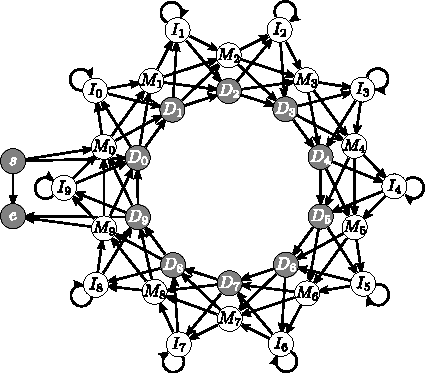
\includegraphics{../figures/SunflowerSilentCircle.pdf}
\caption{Cyclic profile model}\label{SUBFIGURE:SUNFLOWERSILENTCYCLE}
\end{subfigure}%
\begin{subfigure}[b]{0.5\textwidth}
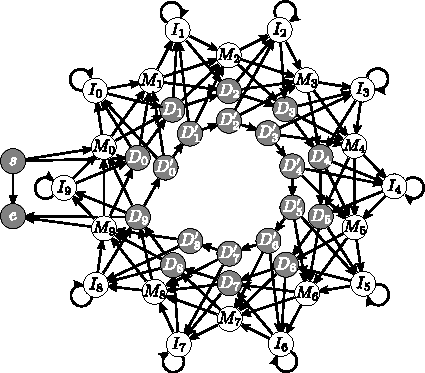
\includegraphics{../figures/Sunflower.pdf}
\caption{Sunflower model}\label{SUBFIGURE:SUNFLOWER}
\end{subfigure}
\end{center}
\caption[Example of the Sunflower model]{Example of the Sunflower model for
consensus of length $10$. White states emits one character and gray states are
silent states. States $s$ and $e$ are initial silent states. Sunflower model
has additional delete states $D'_0, \dots D'_8$ to remove silent cycle from the
model.}
\label{FIGURE:SUNFLOWERMODEL}
\end{figure}

To model this process, start with profile HMM for consensus $C$ and made it
cyclic: It contains states $M_0,\dots, M_{k-1}, I_{0}, \dots, I_{k-1}$ and
$D_{0}, \dots, D_{k-1}$. The transitions between the states are similar to
profile HMM:  $M_{i}\to M_{i\oplus 1}, M_i\to I_i, M_i\to D_{i\oplus 1}, I_i\to
I_i, I_i\to M_{i\oplus 1}, I_i\to D_{i\oplus 1}, D_{i}\to D_{i \oplus 1},
D_{i}\to M_{i\oplus 1}, D_{i}\to I_i$ for all $0\leq i < k$, where $\oplus$ is
$+$ modulo $k$. As in profile HMM, $D_i$ states are silent. Additionally we add
silent start state $s$ and silent end state $e$ with transitions $s\to M_0,
s\to D_0, D_{k-1}\to e, M_{k-1}\to e$ and transition $s\to e$ to model empty
tandem repeat.  Whole model topology is in Figure
\ref{SUBFIGURE:SUNFLOWERSILENTCYCLE}.

The problem with this model is that it contains cycle of silent states, which
causes problems with training and decoding algorithm, as was briefly mentioned
in section \ref{SECTION:SILENT}. We could remove these states, but we would
have to add additional $\theta(k^2)$ edges to by able to delete arbitrary (in
cyclic sense) parts of consensus cycle. Therefore we have decided to remove
transition between delete states $D_{k-1}$ and $D_0$. To compensate to the lost
possibility of deleting arbitrary part of tandem repeat, we add additional
chain of delete states $D'_0, \dots, D'_{k-2}$ that are accessible only from
state $D_{k-1}$ (by transition $D_{k-1}\to D'_0$ and their outgoing
transitions are similar to delete state transitions: $D'_{i}\to M_{i+1},
D'_{i}\to I_i$ for $0\leq i\leq k-2$ and $D'_{i} \to D'_{i+1}$ for $0\leq i <
k-2$. Full model is in Figure \ref{SUBFIGURE:SUNFLOWER}. We call this model the
\firstUseOf{Sunflower} model.

\todo{Premenuj end state na final state, vsade!} This model has $4k+1$ states
out of which $2k+1$ are silent, and $12k+1$ transitions. Since alphabet size is
$4$, there are $14k+2$ parameters to train for a consensus $C$ (including
emissions of insert and match states). Models with large number of parameters
are hard to train, so we reduce the number of parameters. We bind similar
transitions so that they have the same probability.  We ended with parameters
$p_{ab}$ where $a,b\in \{m, i, d, \cdot\}$. $m$ stands for any match state, $i$
stands for any insert state, $d$ states for any delete state (from both
chains), and $\cdot$ is either start or end state. Therefore probability of
transition from match state to delete state is $p_{md}$ and probability of
transition from insert state to final state is $p_{i\cdot}$.  Probabilities
were set in a way, that $\sum_{b\in\{m,i,d\}p_{ab}}=1$ for all possible $a$.
Therefore, transitions from $M_{k-1}, D_{k-1}$ and $D'_{k-1}$ does not sum to
$1$, because they are either missing one transition of having one additional
transition. Therefore for those states the probability of transitions were
multiplied by constant so that they form probability distribution.
\todo{Skontroluj ci tu nie su nejake vynimky}

Emission parameters were reduced in following way: all insert states shared
same emission distribution. For emission distribution of match state $M_i$ we
assumed that base from consensus $c_i$ evolved over evolutionary time $t$
according to Jukes-Cantor model. This model is theoretical model of evolution
that assumes constant rate of evolution. Under this model base $B_1$ evolved
over time $t$ to different base $B_2$  with probability $1/4(1-\exp(-4t/3))$.
The probability that $B_1$ after time $t$ will be again $B_1$ is
$1/4(1+3\exp(-4t/3))$ \cite{Durbin1998}. Time $t$ was same for all match
states. Therefore emissions of all states has only $4$ parameters ($1$ for
match states and $3$ for insert states).

\begin{note}
In Jukes-Cantor model, the parameter $t$ is not time as measured by
seconds/years. It is a branch length in evolutionary tree and it is
multiplication of substitution rate and time. We used this small inaccuracy to
simplify explanation.  More details can be found in \cite{Durbin1998}.

\end{note}

Sunflower model models only tandem repeat and it is not directly usable for
finding tandem repeats. To do so, we have to alter this model. Let $S_C$ be the
Sunflower for consensus sequence $C$. Then we create model consisting of state
$B$, that model non-repetitive part of the sequence with model $S_C$ with an
transition $B\to s$ with probability $p_r$ which is the probability of repeat
starting at particular position in the sequence and with transition $e\to B$
with probability $1$. There is also transition $B\to B$ with probability
$1-p_r$. Afterwards, we can use the Viterbi algorithm with this model to find
all of the occurrences of tandem repeat with consensus $C$. However, with this
model we can search only for specific repeats. We will use this model as an
submodel in following section. 


\section{Models for Aligning with Tandem Repeats}\label{SECTION:REPMODELS}
\begin{reformulate*}
Popiseme nase oba modely. sunflower, a ten tantan-like
Presnejsie:\\
$*$ Ake zhruba ciele mame (mozno do inej kapitoly)\\
%$*$ Popisat to ako 4-stavovy generalizovany model\\
%$*$ Instancia ako SUNFLOWER\\
%$*$ Instancia ako TANTAN\\
%$*$ Expandovanie ciernej skrinky
\end{reformulate*}

In this section we describe models that we have used in our methods. We
describe it in an dual way. As an generalized PHMM and later we extend it into
equivalent PHMM (emissions length are at most $1$ in all sequences).
Equivalency is in the way, that distribution of generated alignments and
annotations are same.

Generalized model is obtained by taking simple three state HMM model from
section \ref{} and adding single generalized pair state $R$, called
\firstUseOf{repeat state}, that in single step generates whole tandem repeats
in both sequences. Since $R$ state can in theory generate arbitrary long
sequences, while decoding using this model, $R$ state does not produce
alignment of bases of tandem repeats. Its aim is to filter tandem repeats out
of alignment so that they do not cause biases in the alignments formed by other
states (match and indel states). To realign those parts later in
post-processing step. The overall topology of GPHMM is illustrated in figure
\ref{FIGURE:REPEAT_GENERAL}.

To made this model flexible, emission distribution of $R$ is defined by
additional PHMM. Since repetitive sequences in tandem repeat are very similar
to each other, we did not try to model the evolution of repetitive part of the
sequence. We assumed that repeats generated by one emissions of $R$ originates
from single consensus sequence and were developed independently. Model was
constructed from sunflower models. Let $C$ be the set of all consensuses that
we want to model. For each consensus $c\in C$ we created sunflowers $S_c^X$ and
$S_c^Y$.  $S_c^X$ is pairwise sunflower model with consensus $c$ that generates
symbols in sequence $X$ and nothing in second sequence. $S_c^Y$ is analogous.
We connect $S_c^Y$ after $S_c^X$ and thus getting model $H_c$ that generates
repeats in both sequences. We connected models $H_c$ for $c\in C$ in parallel
by single start and single end state as in figure \ref{FIGURE:REPEAT_GENERAL}.
The probability from start state to model $H_c$ was determined from posterior
distribution of consensuses $\prob{c}$. Note that the size of this model is
determined mostly by the size of set of all consensuses and therefore this
model can be very large, even infinite if we consider all possible sequences as
an possible consensus for an repeat. To keep the model size small we used
program TRF to compute a set of candidate consensuses $C$ and use it for
construction of model.  We call this generalized model \abbreviation{sunflower
field}{SFF}.

\begin{figure}
\begin{center}
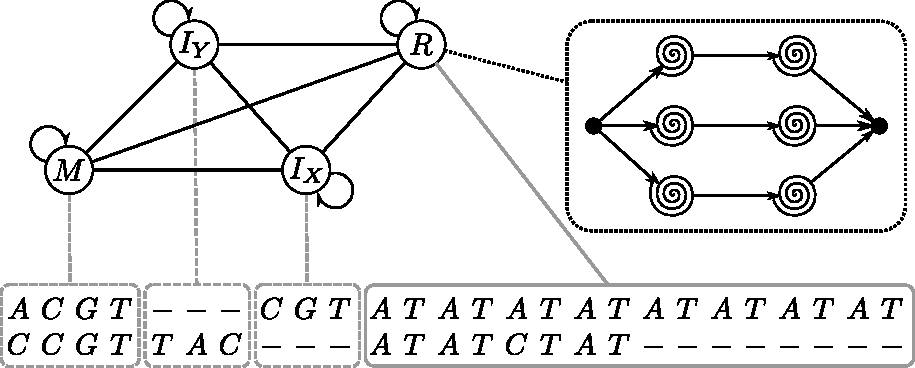
\includegraphics[width=14cm]{../figures/PairRepeatHMMGeneral.pdf}
\end{center}
\caption[General topology of Repeat PHMM]{ 
Topology of Repeat PHMM. We extend 3-state PHMM with one generalized states
$R$, that in one emission generates tandem repeats in both sequences. The
emission distribution of $R$ state is defined by another PHMM. Gray lines
represents emissions: dashed lines corresponds to multiple emissions from same
states, while full line represents one emission. Dotted black line represents
connection to submodel that is used for generating tandem repeats.

Black states in submodel on the right are silent start and end states. Spirals
represents submodels generating tandem repeat in one sequence. They are in
pairs of two identical models, one for generating tandem repeat in one
sequence, other for generating tandem repeat in other sequence. There are
multiple pairs of submodels, each for modeling different consensus.

 }\label{FIGURE:REPEAT_GENERAL} 
\end{figure}

We also experimented with using TANTAN-like model in construction of PHMM
defining emissions distribution of state $R$. Since TANTAN model does not model
the first repetition, we have added chain of states $I_1, \dots, I_n$ to model
first repetition.  Similarly as with sunflowers, we created two copies of
TANTAN, each generating repeats in only one sequence and connect them together
exactly as we would connect sunflowers. Since TANTAN model does not rely on
consensus, it is not necessary to create more copies of TANTAN HMM and it's
general topology looks like SFF's with only one consensus. Since TANTAN is high
order HMM, resulting model is high order and generalized pair HMM. We refer to
this model as \abbreviation{TANTAN PHMM}{TTP}. Advantage of this model over SFF
is in it's size, since TTP will have in practice less states than SFF. However
in TTP, does not satisfy assumption that repeats origins from single consensus,
since each repetitive element is created from previous occurrence and repeats
in sequences $X$ and $Y$ are independent of each other. \todo{obrazok?}

While having SFF or TTP defined as an $4$ state hight order GPHMM might be
convenient for some decoding methods, in general using generalized models
increase time complexity of decoding algorithms quadratically. Therefore we
also worked with their expanded versions: we removed state $R$ and replace it
with model generating repeats (referred as a submodel). All transitions
entering originally into $R$ were directed to start state of submodel and all
outgoing transitions from $R$ now start in end state of submodel. Distributions
of alignments generated by this PHMM has clearly not changed. Additionally, if
in original GPHMM we used identity function as an labeling function
$\lambda_{ID}$ and in expanded model we label states from submodel by label
$R$, resulting in labeling function $\lambda_R$, distribution on annotations
on alignments has also not changed. \todo{toto znie ako od hotentota}

\todo{Ako je definovana pravdepodobnost emisie?}

\begin{comment}
By this we obtained model that 

We started from HMM $H$ that model repeats and alter it to
PHMM, so that it generates empty sequences in one strand. By this we get 2 HMMs
$H_X$ and $H_Y$, first that generates bases only in sequence $X$ and second
that generates bases only in sequence $Y$. 

tandem repeats together, just label them that they 
\begin{itemize}
\item Reduce alignment alignment error near repeats
\item Improve alignment of the repeats
\end{itemize}
We kept in mind following \reformulate{???} while designing model:
\begin{itemize}
\item We assume star phylogeny of the repeats: all repetitions of repeat evolved
from single consensus sequence independently.
\item We want to label repetitive regions.
\item Correct alignment of two repetitive regions is very hard, if not
impossible. This is because these regions are very similar \todo{Chcelo by to
vygenerovat graf, sekvencnej identity, poctu insertov a podobne ako funkciu vo
vzdialenosti od repeatu}.
\end{itemize}


We have two models, sunflower and TANTAN-like model. They both differ
significantly in how they treat consensus.

The main model is similar to standard 3-state model for pair alignments. We
have added  submodel modeling repeats. All states in the submodel had same
label. Repeats were modeled in each sequence independently, so basically to
model repeats, we have chained model for repeats in sequence $X$ and model for
repeats in sequence $Y$. We did not try to model evolution of the repeats due
to the high sequence similarity of repeats.  We do not believe that there is
enough information in the repeats (and errors in them) to practically improve
the alignments of the repeat parts. On the other hand, this model produces
alignments where all repetitions were indels, which is not realistic. To cope
with this drawback, we realigned repetitive parts along with flanking
insertions by simple 3-state HMM.

While the TANTAN model models repeats of any sequences, we could just have one
copy of TANTAN model for sequence $X$ and one copy for sequence $Y$.  However,
for the sunflower submodel, each sunflower models only repeats of one specific
sequence, therefore we can model only one possible repetitive sequence by using
only one\footnote{Two same sunflowers for both sequences.} sequence. To
overcome this very strict constrained, we have to one sunflower per consensus
we want to model. We put sunflowers together in parallel way, so that they are 
Topology of both of these models are described in figure \ref{}.

\end{comment}

\section{Decoding methods}
\begin{reformulate*}
Tu popiseme ake dekodovacie metody pozname: viterbi, posterior, block \{viterbi,
posterior\}
Presnejsie:\\
$*$ Viterbi\\
$*$ Posterior (marginalized aj nie)\\
$*$ Block viterbi\\
$*$ Block posterior\\
\end{reformulate*}

In this part we describe several optimization criteria we have used. We used
following optimization criterias/algorithms: the Viterbi algorithm (VA), the
posterior decoding (PD), the marginalized posterior decoding (MPD), block
Viterbi algorithm (BVA) and block posterior decoding (BPD). The first three
methods we used with expanded models, the latter two methods we used with
generalized version of the model.

\todo{Zopakuj gain funkcie, nech vieme co optimalizujeme}

Whenever in this chapter we refer to VA, PD, MPA, we mean algorithms from
chapter \ref{} applied to algorithms applied to expanded version of SFF or TTP.
BVA is Viterbi algorithm applied to non-expanded SFF or TTP. Block posterior
decoding is however different. Problem is that posterior probabilities of
emissions from generalized states are much smaller than from regular states,
because they are much longer. Since the posterior probabilities are much lower,
non-generalized states will be favored in the resulting alignment. Therefore 
we added compensation element for generalized states, to level playing field.
We have multiplied the posterior probability with the number of bases within
such emissions. Therefore gain function for BPD is following: We add +1 for
every base, that is aligned with base/gap that was generated by same state as
in the original alignment.
\todo{Sem chcem dodat detaily, ale asi az po tom, ako prepisem 4-tu kapitolu a
zakomponujem bronine poznamky + pridat casove zlozitosti}


\section{Implementation details \& optimizations}
\begin{comment}
\begin{reformulate*}
Implementacne detaily, optimalizacie, cachovanie
Presnejsie:\\
$*$ Banding, \\
$*$ Konsenzy -- TANTAN vs SFF\\
$*$ ako sa cachovali, spomenut ze ake rozne optimizacne kriteria by to mohlo mat\\
$*$ Ako sa vyberali hinty pre block viterbi
\end{reformulate*}
\end{comment}

To reduce processing time, we implemented following optimizations:
\begin{itemize}
\item Banding: at first we align sequences using Muscle\cite{} to get guide
alignment. We explore only alignments that were within 30 bases from the guide
alignment.

\item TTP does is not dependent on consensus, however size of SFF is. Therefore
we have used TRF program to find all candidate consensuses in input sequences
and uses only those consensuses to build SFF.

\item When using generalized models, time complexity of the decoding methods is
very large.  Therefore to compensate for this drawback, we used TRF program to
get list of candidate intervals where tandem repeats could occur. We use this
intervals to restrict parts of the sequence where the repeat state $R$ could be
used. Since TRF tool is not perfect in finding tandem repeats, ...

\item When using gadget that generated tandem repeats for particular consensus,
we run submodels independently on each sequence and cached results to prevent
from computing same information twice. In actual implementation, we at first
computed all emissions of $R$ state before we start computing posterior
probabilities. We did this because when computing probability of something, you
can also probability of all prefixes.  By this way we had guaranteed that all
of the computation were done in correct order.

\end{itemize}

\section{Experiments}
\begin{reformulate*}
Ako sa generovali data, ako sa trenovali modely, ake miery sledujeme.  Bolo by
zaujimave sa pozriet ako porovname s hladanim tandemovych repeatov ak pouzijeme
TRF, alebo sunflower.

\end{reformulate*}

To evaluate our approach, we do simulation experiment. At first we build model
resembling human-dog alignment. Then we sampled alignments 200 test and 200
train alignments. We trained model on training sample, evaluated several algorithms
on the test set. In this section we summarize details of this experiment and 
measures we were \reformulate{looking at}.


\paragraph{Measures:} The first measure we use was the error rate on the
alignments: number of incorrectly predicted columns of an alignment. Other
measures we investigate were measuring precision of repeat annotation. Therefore 
we were measuring the specificity and sensitivity of repeat labeling of columns
and specificity and sensitivity of identifying the correct repeat block (block
is consecutive sequence of columns, block must have been identical to be
counted as an correctly predicted).

\section{Results}
\begin{reformulate*}
Tabulky, grafy, ... -- presnejsie tabulka, graf
\end{reformulate*}

\section{Possible Improvements}

\begin{reformulate*}
Sem by som mohol napisat, ako by sa dal pouzit symetricky model s cyklom
stavov, alebo ako by sa dal ten cyklus stavov odstranit odstranenim jednej
hrany a pridanych n hran -- co je lepsie ako pridat n vrcholov.
\end{reformulate*}

\label{LastPage}
